\documentclass{beamer}
\usepackage{listings}
\usepackage{amsmath,amssymb,amsfonts}
\usepackage{graphicx}
\usepackage{hyperref}
\usepackage{textcomp}
\usepackage{xcolor}
\usepackage{algorithm}
\usepackage{algorithmic}
\usepackage{geometry}
\usepackage{array}


\title{Group 3:\\LDPC Codes in Computer Memory}
\author{Tom Wang\\Natalie Balashov}
\date{April 11th, 2024}

\begin{document}

\begin{frame}
    \titlepage
\end{frame}

\begin{frame}{Overview}
    \begin{enumerate}
        \item Applications of Codes in Memory
        \item Introduction to LDPC Codes
        \item Implementation of LDPC Codes in HDL
        \item Implementation of Hamming Codes in HDL
        \item Comparison of LDPC and Hamming Codes
    \end{enumerate}
\end{frame}

\begin{frame}{Application Codes in Computer Memory}
  \begin{itemize}
    \item Error-correcting codes in memory systems are crucial to maintaining data integrity.
    \item With increasing memory densities and memory chip sizes, bit errors occur more frequently.
    \item Special technologies like spin-torque transfer random access memory (STT RAM) experience asymmetric bit errors.
    \item Niche applications like space missions require more robust error-correction strategies due to overly noisy channels created by radiation.
    \item In addition to performance and error-correcting capacity, hardware resources are a design constraint.
  \end{itemize}
\end{frame}

\begin{frame}{Low-Density Parity Check (LDPC) Codes}
  \begin{itemize}
    \item LDPC codes are linear block codes characterized by sparse parity check matrices.
    \item LDPC codes have been shown to achieve near Shannon capacity performance.
    \item First proposed by Gallager in 1960, as part of his Ph.D. thesis.
    \item Two main types: regular and irregular.
    \item A LDPC code with parameters $(n,j,i)$ has a block length $n$, $j$ ones in each column of $H$ and $i$ ones in each row of $H$.
  \end{itemize}
\end{frame}

\begin{frame}{LDPC Parity Check Matrix}
  We examined the LDPC code with parameters $n=72, j=2$ and $i=18$.\\
  \medskip
  This particular matrix was generated with the Python library \texttt{pyldpc}, which uses the typical algorithm.

  \begin{figure}[htbp]
      \centerline{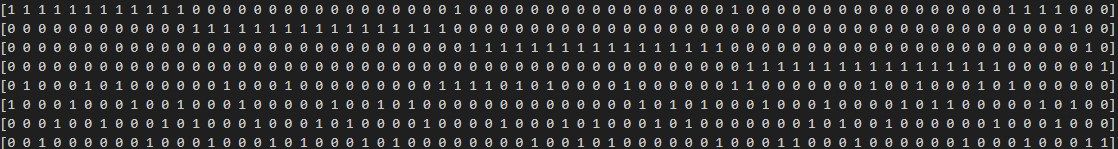
\includegraphics[scale = 0.4]{Images/LDPC_Parity_Matrix.jpg}}
      \caption{8$\times$72 Parity check matrix for LDPC code.}
  \end{figure}
\end{frame}

\begin{frame}{LDPC Generator Matrix}
    To generate the generator matrix, we used the following algorithm:
    \begin{enumerate}
      \item Re-organize the codeword $\textbf{c}$ of length $n$ so that it is of the form $\textbf{c} = [\textbf{b}, \textbf{m}]$, where $\textbf{b}$ denotes the parity bits vector and $\textbf{m}$ denotes the message bits vector.
      \item Sub-divide the parity matrix $H$ into two sub-matrices such that $H = [H_1, H_2]^T$ where $H_1$ is a square matrix of size $n-k$.
      \item Since $\textbf{b}$ is of length $n-k$ as well, we can break up the matrix
    multiplication into $[\textbf{b}, \textbf{m}][H_1, H_2]^T = \textbf{b}H_1^T + \textbf{m}H_2^T = 0$.
    \item Since we are dealing with a code defined on a binary field, $\textbf{b}H_1^T = \textbf{m}H_2^T$ implies that $\textbf{b}= \textbf{m}H_2^T(H_1^T)^{-1}$.
    \item With $A = H_2^T(H_1^T)^{-1}$, the generator matrix $G$ is $[A, I_{n-k}]$.
    \end{enumerate}
\end{frame}

\begin{frame}{LDPC Decoding Algorithm}
  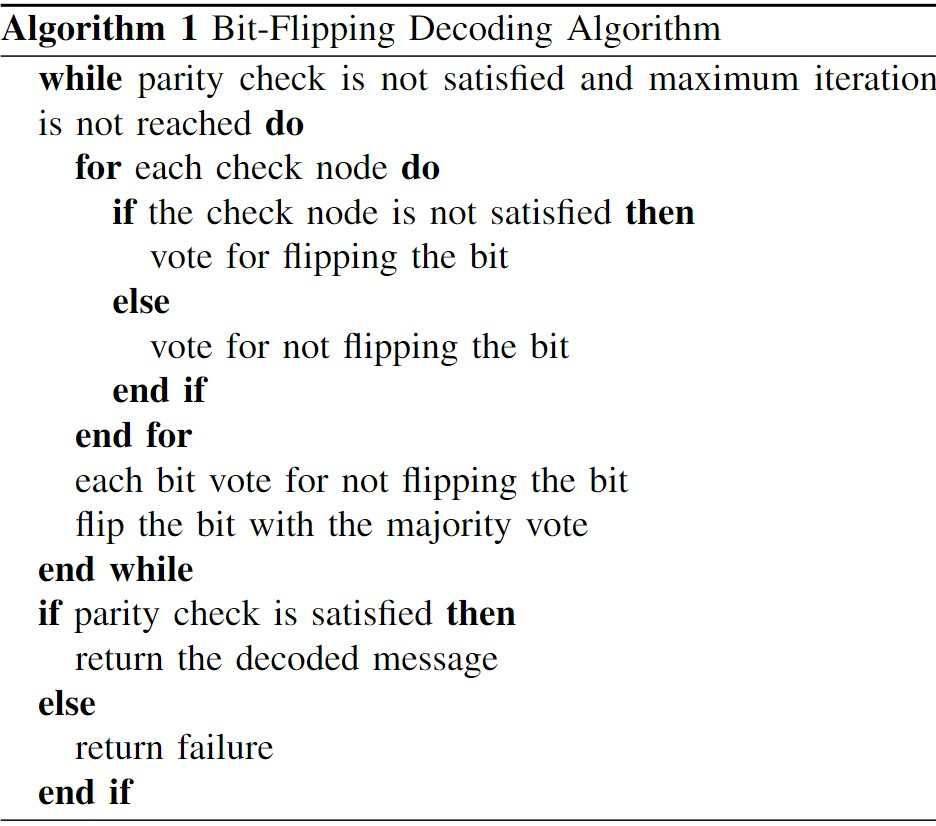
\includegraphics[scale=0.3]{Images/Bit_Flipping_Algorithm.jpg}
\end{frame}

\begin{frame}{LDPC Performance}
  On DE1-SOC, Quartus analysis shows that the highest possible clock frequency is \textbf{325.73 MHz}.

  \begin{itemize}
    \item Combinational ALUT usage for logic: 114 \begin{itemize}
      \item 7 input functions: 0
      \item 6 input functions: 4
      \item 5 input functions: 10
      \item 4 input functions: 28
      \item $\leq$ 3 input functions: 72
    \end{itemize}
    \item Dedicated logic registers: 72
  \end{itemize}
\end{frame}

\begin{frame}{Hamming Implementation}
  \begin{itemize}
    \item Typical Hamming code implementation uses 64-bit to 72-bit encoding schemes.
    \item This typical implementation is called Single Error Correction,
    Double Error Detection (SECDED) Hamming code, where the parity bits indicate the index of the bit error.
  \end{itemize}
  \begin{figure}[htbp]
    \centerline{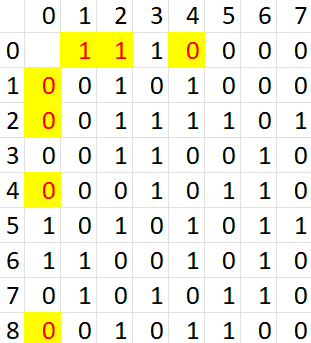
\includegraphics[scale = 0.6]{Images/Hamming_example.png}}
    \caption{Parity bits and data bits in a Hamming code.}
  \end{figure}
\end{frame}

\begin{frame}{FPGA Implementation}
    Logic can be easily achieved with a combination of AND gates and XOR gates.

    According to Quartus timing analysis, the highest possible clock frequency is
    \textbf{387.3 MHz}.

    \begin{itemize}
      \item Combinational ALUT usage for logic: 154
      \begin{itemize}
        \item 7 input functions: 0
        \item 6 input functions: 121
        \item 5 input functions: 10
        \item 4 input functions: 13
        \item $\leq$ 3 input functions: 10
      \end{itemize}
      \item Dedicated logic registers: 69
    \end{itemize}
\end{frame}

\begin{frame}{Comparison}
  \begin{table}[htbp]
    \centering
    \caption{Comparison of Decoding Algorithms}
    \label{tab:decoding_comparison}
    \begin{tabular}{|l|c|c|}
      \hline
      \textbf{Parameter} & \textbf{Hamming} & \textbf{LDPC} \\
      \hline
      Highest Frequency (MHz) & 387.3 & 325.73 \\
      \hline
      ALUT Usage for Logic & 154 & 114 \\
      \quad 7 input functions & 0 & 0 \\
      \quad 6 input functions & 121 & 4 \\
      \quad 5 input functions & 10 & 10 \\
      \quad 4 input functions & 13 & 28 \\
      \quad $\leq$ 3 input functions & 10 & 72 \\
      \hline
      Dedicated Logic Registers & 69 & 72 \\
      \hline
    \end{tabular}
  \end{table}
\end{frame}

\begin{frame}{Conclusion}
  \begin{itemize}
    \item Hamming code can operate at a higher clock frequency.
    \item LDPC code has a lower ALUT usage and more dedicated logic registers.
    \item LDPC code uses significantly fewer 6-input function blocks.
    \item This means that the LDPC code is more efficient in terms of hardware usage.
    \item The frequency difference is not significant. On ASIC designs, the performance comparison might be different. 
  \end{itemize}
\end{frame}

\end{document}
